\chapter{Graph-based map analysis}

% INTRODUCTION %

In this chapter we describe the approach that we have developed to perform analysis and populating of pre-generated maps using \<Graph Theory>. After a quick overview, we introduce the analysis capabilities of this approach and then we present how we employed it to strategically place game elements in pre-generated maps.

% DESCRIPTION %

\section{Overview}

Our approach consists of generating different kind of graphs, starting from the text and the All-Black representation of a map, that are used to perform various analysis and manipulation operations.

\par

The use of All-Black format is convenient, because it provides by default a logical division of the map in different areas and it allows our approach to be applied by other researchers, since as we have seen the All-Black format is widely used in the literature. In this thesis we focused on positioning objects in pre-generated maps, but, for instance, the same approach could be used to address the identification and definition of design patterns from an unfamiliar perspective or for \<direct evaluation> in Search Based PCG.

% ANALYSIS %

\section{Analysis of the map}

The analysis is performed by generating different kind of undirected graphs, each one used to highlight a different feature of the map in question, using a \<Python> tool based on \<NetworkX>\footnote{A solid graph theory library (\url{https://networkx.github.io/}).} that we developed.

\subsection{Outlines graph}

The \<outlines graph> is generated starting from the All-Black representation of a map and is obtained by associating a node to every vertex of every room and corridor and by connecting the non-adjacent ones that belong to the same outline. This graph has a single kind of node (\<vertex node>) that contains the coordinates of the tile it represents, which are used to position the node when the graph is visualized. Figure \ref{img:graph_out} shows an example of this graph. This graph can be used to visualize the rooms which compose the map.

\subsection{Reachability graphs}

Our tool can generate various kinds of \<reachability graphs> that represent various ways in which it is possible to navigate the map. In these graphs a node represents a reachable position, whereas an edge indicates a viable path from a position to another.

\subsubsection{Tiles graph}

The \<tiles graph> is generated starting from the text representation of a map and is obtained by associating a node to each empty tile and by connecting each node to its 8-neighbors. The horizontal and vertical edges have cost $1$, whereas the diagonal ones have cost $\sqrt{2}$. This graph has a single kind of node (\<tile node>) that contains the coordinates of the tile it represents, which are used to position the node when the graph is visualized. Figure \ref{img:graph_tile} shows an example of this graph. This graph can be used to find the minimum distance that separates two cells, along with the shortest path that connects them.

\subsubsection{Rooms graph}

The \<rooms graph> is generated starting from the All-Black representation of a map and is obtained by associating a node to each room and corridor and by connecting nodes which corresponding rooms or corridors overlap, using as weight the Euclidean distance of their central tile. This graph has a single kind of node (\<room node>), used to represent both rooms and corridors that contains the coordinates of the closest and furthest vertex of the room from the origin. When visualized, each node is positioned on the coordinates of the central tile of the room it represents. Figure \ref{img:graph_room} shows an example of this graph. This graph can be used to analyze the topology of a map, in order to find loops, choke points, central areas and other kind of structures.

\subsubsection{Rooms and game elements graph}

The \<rooms and game elements graph> is an extension of the rooms graph, which also includes game elements as nodes, that are connected to the nodes corresponding to the rooms and corridors which contain them. In addition to the room node inherited form the rooms graph, this graph has a node to represent game elements (\<element node>) that contains the coordinates of the game element, which are used to visualize the node, and the character associated to the it. Figure \ref{img:graph_room_res} shows an example of this graph.

\subsection{Visibility graph}

The \<visibility graph> is generated starting from the text representation of a map and is obtained by associating a node to each empty tile and by connecting each node to all the tiles that are visible from that node. For two tiles to be respectively visible, it must be possible to connect them with a line without crossing any filled tile. This graph has a single kind of node (\<visibility node>) that contains the coordinates of the tile it represents, which are used to position the node when the graph is visualized, and its \<visibility>, which is computed as the \<degree centrality>, i.e. the number of edges incident to that node. A tile with high visibility allows to control a wide portion of a map, but at the same time an entity standing on it is easy to spot.

\par

To make this graph easier to read by the user, the tool associates a color to the nodes, which ranges from blue, for the ones with the minimum visibility, to red, for the ones with the maximum visibility. This can be seen in figure \ref{img:graph_visibility}. This graph can be used to analyze which areas of the map are more exposed and which ones are more repaired.

\begin{figure}[]
	\centering
	\hfill
  	\begin{subfigure}[t]{0.45\linewidth}
		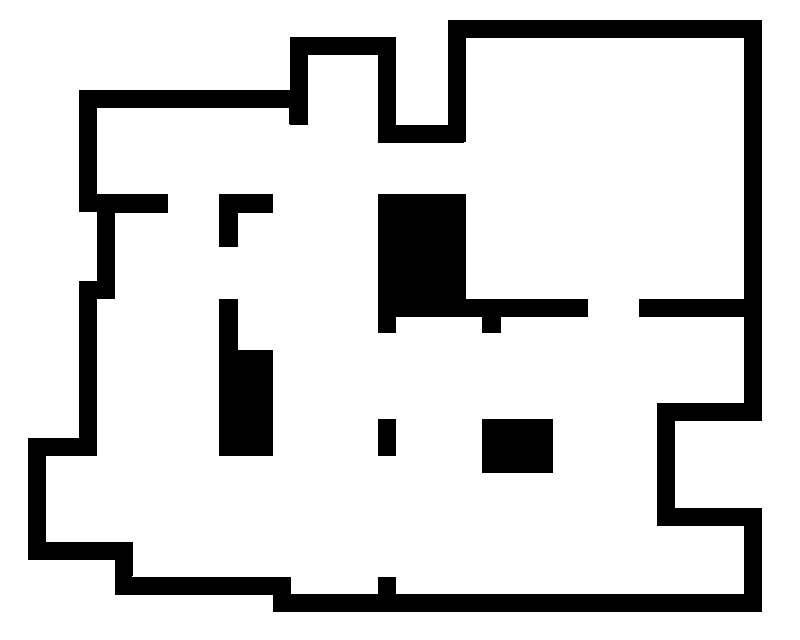
\includegraphics[width=\linewidth]{graph_divisive}
     		\caption{The map.}
     		\label{img:graph_divisive}
 	\end{subfigure}
 	\hfill
  	\begin{subfigure}[t]{0.45\linewidth}
    		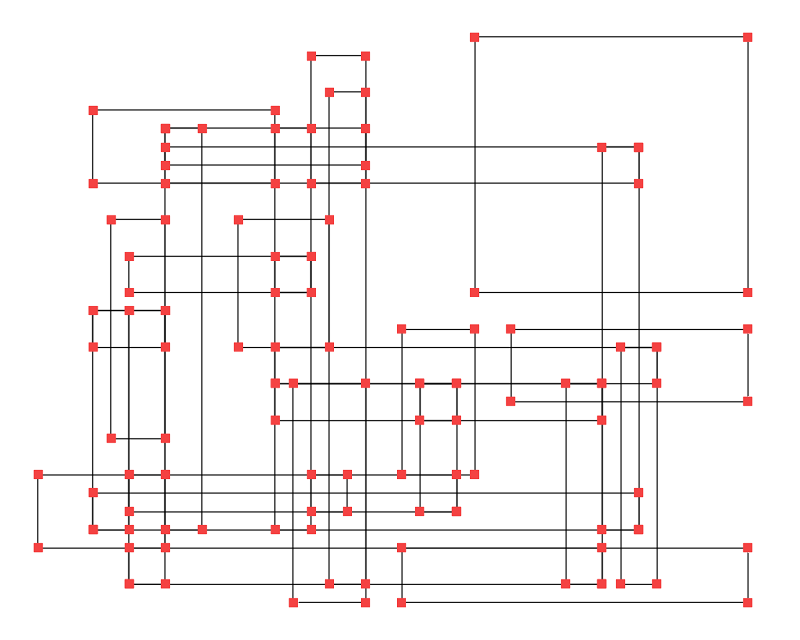
\includegraphics[width=\linewidth]{graph_out}
    		\caption{The outlines graph of the map.}
     		\label{img:graph_out}
  	\end{subfigure}
  	\hfill
  	
  	\hfill
  	\begin{subfigure}[t]{0.45\linewidth}
    		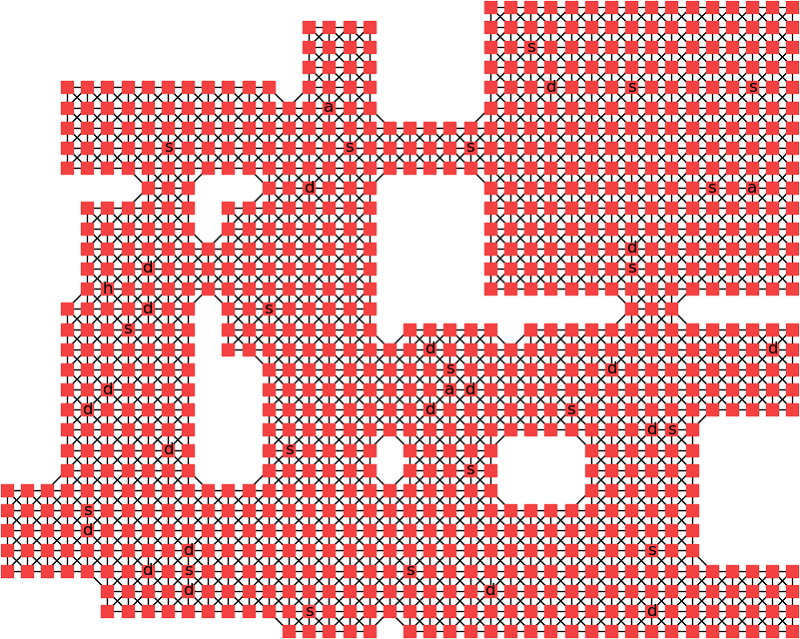
\includegraphics[width=\linewidth]{graph_tile}
    		\caption{The tiles graph of the map.}
     		\label{img:graph_tile}
  	\end{subfigure}
  	\hfill
  	\begin{subfigure}[t]{0.45\linewidth}
    		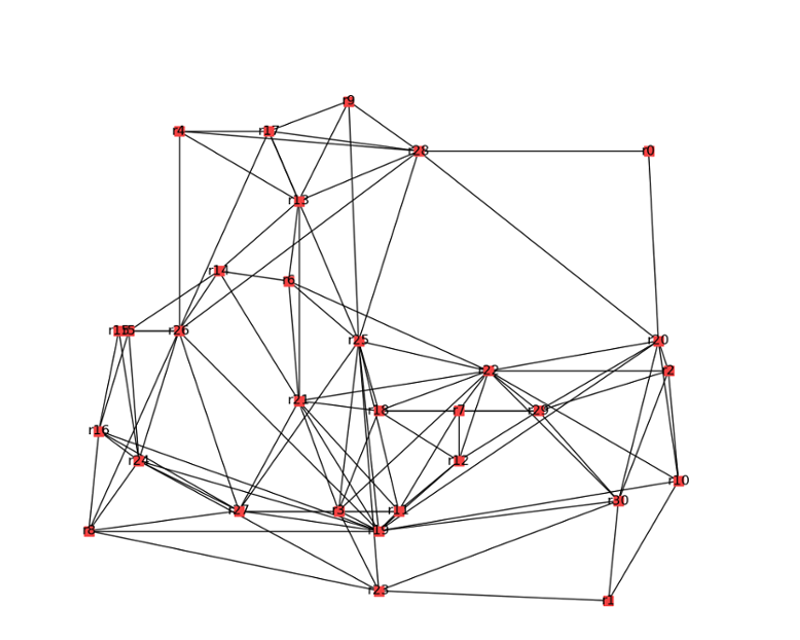
\includegraphics[width=\linewidth]{graph_room}
    		\caption{The rooms graph of the map.}
     		\label{img:graph_room}
 	\end{subfigure}
 	\hfill
 	
 	\hfill
  	\begin{subfigure}[t]{0.45\linewidth}
    		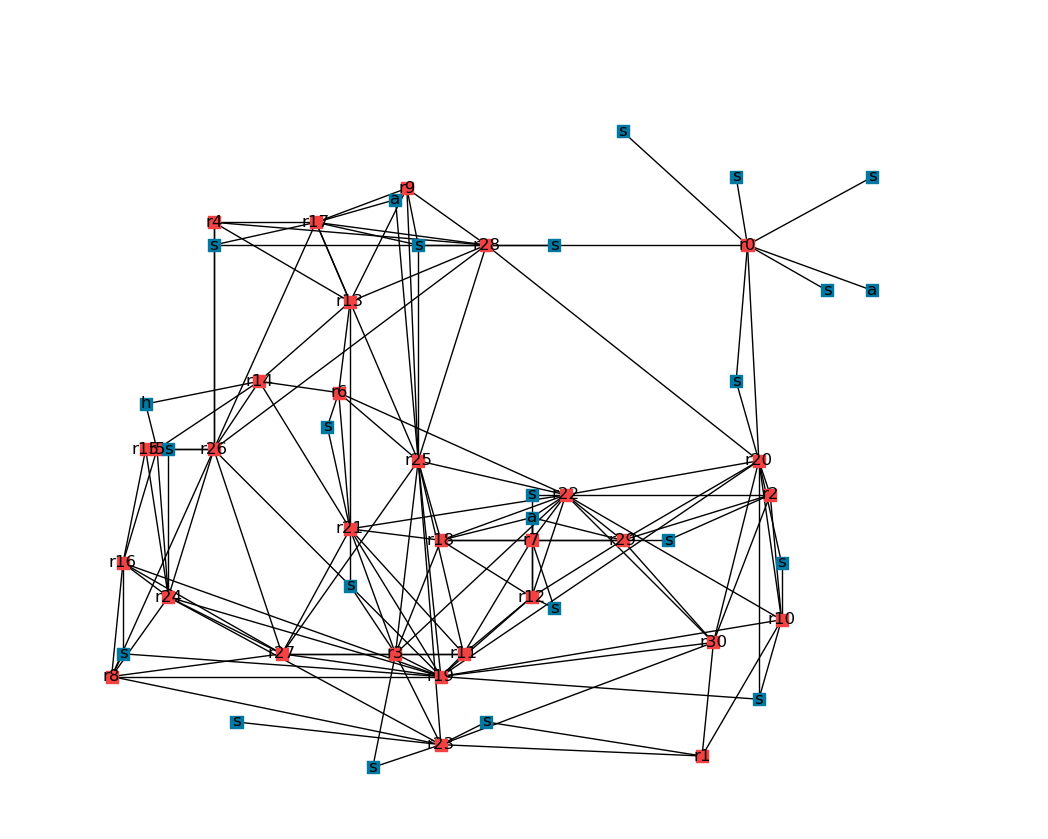
\includegraphics[width=\linewidth]{graph_room_res}
    		\caption{The rooms and game elements graph of the map.}
     		\label{img:graph_room_res}
  	\end{subfigure}
  	\hfill
  	\begin{subfigure}[t]{0.45\linewidth}
    		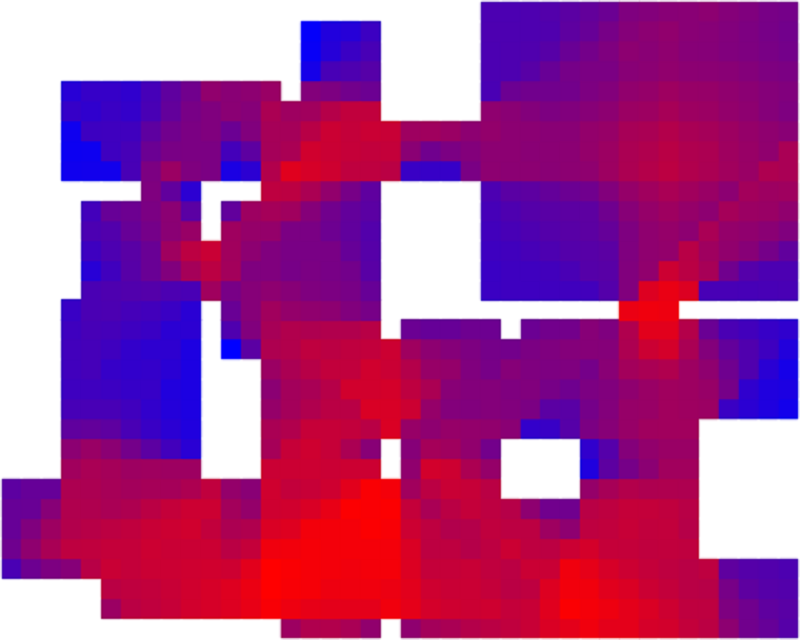
\includegraphics[width=\linewidth]{graph_visibility}
    		\caption{The visibility graph of the map.}
     		\label{img:graph_visibility}
  	\end{subfigure}	
  	\hfill
	\caption{A map and all the graphs that can be generated from it.}
\end{figure}

\subsection{Interesting metrics}
\label{ss:interesting_metrics}

Considering the graphs, in particular the ones with room nodes, the following metrics defined by Graph Theory provide interesting information about the layout of a map:

\begin{itemize}
\item \<Degree centrality>: defined for a node, it is the number of edges that the node has. If the node represents a room, it measures how many entrance or exits the room has. 
\item \<Closeness centrality>: defined for a node, it measures its centrality in the graph, computed as the sum of the lengths of the shortest paths between the node and all other nodes in the graph. If the node represents a room, it measures how central the room is.
\item \<Betweenness centrality>: defined for a node, it measures its centrality in the graph, computed as the number of shortest paths connecting the nodes that pass through the node. If the node represents a room, it measures how central the room is.
\item \<Connectivity>: defined for a graph, it is the minimum number of elements (nodes or edges) that need to be removed to disconnect the remaining nodes from each other. If the graph represents a map, it measures the existence of isolated areas.
\item \<Eccentricity>: defined for a node, it is the maximum distance from the node to all other nodes in the graph. If the node represents a room, it measured how isolated the room is.
\item \<Diameter>: defined for a graph, it is the maximum eccentricity of its nodes. If the graph represents a map, it measures the size of the map.
\item \<Radius>: defined for a graph, it is the minimum eccentricity of its nodes. If the graph represents a map, it measures how distanced the rooms are from each other.
\item \<Periphery>: defined for a graph, it is the set of nodes with eccentricity equal to the diameter. If the graph represents a map, it defines its peripheral areas.
\item \<Center>: defined for a graph, it is the set of nodes with eccentricity equal to the radius. If the graph represents a map, it defines its central areas.
\item \<Density>: defined for a graph, it ranges from 0 to 1, going from a graph without edges to a complete graph. If the graph represents a map, it measures how complex it is.
\end{itemize}

% POPULATING %

\section{Placement of game elements on the map}

We have defined multiple heuristics to populate a map with game elements using the metrics that can be extracted from a graph. These heuristic are a mathematical transposition of rules and patterns concerning game elements placement that we have extracted from the work of Tim Schäfer\cite{great1vs1}, who has performed an in depth analysis of multiplayer 1vs1 maps for \<Quake 2>\footnote{Id Software, 1997}.

\subsection{Rules for the placement of game elements}

The balance of a deathmatch game radically changes each time that a player is killed. If the game has more than two players, the player who won the fight does not gain any strategic advantage, since he still has the other players to face, whereas the defeated player is put at considerable disadvantage, because on death he loses all the weapons and ammunition that he has collected. In a 1vs1 match, a kill has an even stronger influence, since the surviving player has more weapons and ammunition and gains the complete control of the map, that comes with the chance of scoring another easy kill, as soon as the other player respawns, or of searching for additional equipment. Schäfer refers to the surviving player as \[up-player] and to the defeated one as \[down-player].

\par

To design a multiplayer map that is interesting and fun to play, it is important to consider the up-player vs down-player dynamic both when defining the map layout and when positioning game elements.

\par

The spawn points, i.e. the locations where the down-player reappears, should be positioned in areas that are of low interest for the up-player and that are easy to leave. Obviously, central hubs and dead ends are a bad choice, whereas rooms with 2 or 3 exits are usually the best option. 

\par

For what concerns the resources, they must be placed considering both the up-player vs down-player dynamic and the characteristics of the resource itself. It is important to place the right amount of resources on the map, because too many would eliminate the need for exploration, whereas too few would disadvantage the down player. It is also important not to place too many powerful items in the same area or in boring spots, since the risk to obtain them should always be proportional to the strategical advantage they allow to achieve. It is important to consider that a powerful resource is interesting for both players, so it often acts as a \<point of collision>. The resources usually are of five kinds: health packs, \<armors>, \<power-ups>, ammunition and weapons. 

\par

The health packs are placed in zones that are safe or not too dangerous. They have no use for the down-player, that respawns with full health, but they can be useful for the up-player, if he has been damaged during the fight, whereas they always come in handy during a fight or after that one of the contenders disengages.

\par

Armors, which supply a second health that is consumed before the main one, are usually placed in spots that are aimed both at the down-player and at the up-player: objects that provide a small quantity of armor should be easy to achieve, whereas the ones that provide full armor should be placed in dangerous areas.

\par

Power-ups grant temporary advantages to the player who collects them, like invisibility or increased damage, and are placed in locations difficult to reach and contextual to their effect.

\par 

The position of a weapon and of its ammunition depends on the weapon itself. We can divide the weapons in three categories: \<weak>, \<medium> and \<strong>. Weak weapons are of a certain interest for the down-player, if he has not collected any other weapon yet, and of no interest for the up-player, so they are placed near spawn-points or in gaps where no other weapon is available, together with their ammunition. Medium weapons are of high interest for the down-player, since he needs to get one of them as soon as possible if he wants to face the up-player, so they are placed in areas that are easy to reach and the same goes for their ammunition. Finally, the strong weapons should be placed in areas that are strategically disadvantageous, like dead ends or vertically dominated areas, or difficult to reach. If a weapon is very contextual, i.e. it is useful in very few situations, it is usually placed in an area that allows to take advantage of its features, whereas a weapon that is strong in almost any situation is usually placed in an area where it cannot be used optimally (e.g. a rocket launcher in a small room).

% PLACEMENT PROCESS % 

\subsection{Placement process}
\label{ss:placement}

Starting from these considerations, we defined a process that allows to position any kind of game element in two steps: the selection of a room and the selection of a tile inside the room. This process can be repeated as many time as needed, after having updated the graphs with the newly added game element.

% ROOM %

\subsubsection{Room selection}
\label{sss:room_selection}

The selection of a room can be heuristic-based, uniform or random.

% HEURISTIC ROOM %

\paragraph{Heuristic-based room selection} 

This method selects rooms considering three suitability criteria:

\begin{itemize}
\item \<Degree heuristic>: defined by the function $D(r)$, where $r$ is a room node, it measures how much the degree centrality of the node matches the desired one.
\item \<Game element closeness heuristic>: defined by the function $H_e(r)$, where $r$ is a room node, it measures how much the closeness of the node to the already placed element nodes matches the desired one.
\end{itemize}

Given the rooms and game elements graph of a map ($G_{rr}$) and the subset of room nodes ($R \subseteq G_{rr}$), the room node which is selected is the one which maximizes the following weighted sum of functions:

\begin{align}
r^* = \argmax_{r \in R} (w_D  \times D(r) + w_{H_e}  \times H_e(r))
\label{eq:room_heuristic}
\end{align}

\noindent
The weights $w_D$ and $w_{H_e}$ allow to define how much each one of the two heuristics influences the selection of a room. Both functions should be defined to output a value in the range $[0,1]$, in order to have the same influence for equal weight.

% UNIFORM ROOM %

\paragraph{Uniform room selection} 

This method selects rooms that are uniformly distributed in the map. The first room is selected at random, then, given the rooms and corridors graph ($G_{rr}$), the subset of room nodes ($R \subseteq G_{rr}$) and the subset of element nodes ($S \subset G_{rr}$), the remaining rooms are selected with the following heuristic:

\begin{align}
	r^* = \argmax_{r \in R} ( \min_{s \in S} (\spl(r, s) ))
	\label{eq:tile_heuristic}
\end{align}

\noindent
where $\spl(n, m)$ denotes the length of the shortest path that connects the two nodes $n$ and $m$, found using Dijkstra's algorithm.

% RANDOM ROOM %

\paragraph{Random room selection} 

This method simply selects rooms at random.

% TILE %

\subsubsection{Tile selection}

The selection of a tile can be heuristic-based, uniform or random.

% HEURISTIC TILE %

\paragraph{Heuristic-based tile selection} 

This method selects tiles considering three suitability criteria:

\begin{itemize}
\item \<Visibility heuristic>: defined by the function $v(t)$, where $t$ is a tile node, it measures how much the visibility of the corresponding tile matches the desired one.
\item \<Wall closeness heuristic>: defined by the function $H_w(t)$, where $t$ is a tile node, it measures how much the proximity of the corresponding tile to the walls matches the desired one.
\item \<Game element closeness heuristic>: defined by the function $H_e(t)$, where $t$ is a tile node, it measures how much the proximity of the node with already placed element nodes matches the desired one.
\end{itemize}

Given $G_v$ the visibility graph and $T \subset G_v$ the subset of tiles contained by the selected room, the tile which is selected is the one which maximizes the following weighted sum of functions:

\begin{align}
t^* = \argmax_{t \in T} (w_v \times v(t) + w_{H_w}  \times H_w(t) + w_{H_e}  \times H_e(t))
\end{align}

\noindent
The weights $w_v $, $w_{H_w}$ and $w_{H_e}$ allow to define how much each one of the three heuristics influences the selection of a tile. All three functions should be defined to output a value in the range $[0,1]$, in order to have the same influence for equal weight.

% UNIFORM TILE %

\paragraph{Uniform tile selection} 

This method selects tiles that are uniformly distributed in the room. If no game element has been placed, the central tile is selected, otherwise it is picked out the one that maximizes the distance from the already positioned game elements but is not too close to the walls.

% RANDOM TILE %

\paragraph{Random tile selection} 

This method simply selects tiles from the room at random.

% HEURISTICS %

\subsection{Heuristics for the placement of game elements}

Depending on how a game element needs to be placed inside the map, we have defined different heuristics to perform heuristic-based selection of rooms and tiles.

% SPAWN POINTS %

\subsubsection{Spawn points}
\label{sss:sph}

For spawn points, the heuristic-based approaches for rooms and tiles respectively select rooms that have a small number of connections, are not dead ends and are distant from each other and tiles that offer the best balance between low visibility and distance from the walls. In this way spawn points are placed in passageways that are sheltered and easy to leave. 

% ROOM %

\paragraph{Room selection}

Considering equation \ref{eq:room_heuristic} and given the rooms and game elements graph of the map ($G_{rr}$ ), the subset of room nodes ($R \subseteq G_{rr}$ ) and the subset of element nodes ($S \subset G_{rr}$), the most suitable room for containing a spawn point is selected using the following heuristics:

\begin{align}
\label{eq:lowriskdeg}
D(r) = \begin{cases}
    		\hfil 0 & \text{if } \degcent(r) = 1 \\
    		1 - \cfrac{\degcent(r) - \min_{r' \in R}\degcent(r')}{\max_{r' \in R}\degcent(r') - \min_{r' \in R}\degcent(r')} & \text{if } \degcent(r) \neq 1 \
  	\end{cases}
\end{align}

\begin{align}
\label{eq:lowriskres}
H_e(r) = \min_{n \in G_{rr}}
  	\begin{cases}
    		\hfil 1 & \text{if } n \notin S \\
    		\cfrac{\spl(r, n)}{\diam(G_{rr})} & \text{if } n \in S \
  	\end{cases}
\end{align}

\noindent
where $\degcent(n)$ denotes the connectivity degree of the node $n$ and $\diam(G)$ the diameter of the graph $G$. Equation \ref{eq:lowriskdeg} promotes rooms with few passages but that are not dead ends, whereas equation \ref{eq:lowriskres} promotes rooms that are distant from the already placed game elements. Both are normalized in the range $[0,1]$. We empirically set the weighs to $w_D = 1 $ and $ w_{H_e} = 0.5 $.

% TILE %

\paragraph{Tile selection}

Considering equation \ref{eq:tile_heuristic} and given the visibility graph of the map ($G_v$), the subset of tile nodes that belong to the room ($T \subset G_v$), the subset of tile nodes of the room which contain a game element ($H \subset T$) and the length of the diagonal of the room  ($l_d$), the most suitable tile for containing a spawn point is selected using the following heuristics:

\begin{align}
\label{eq:lowvis}
v(t) = 1 - \cfrac{\degcent(t) - \min_{t' \in G_v}\degcent(t')}{\max_{t' \in G_v}\degcent(t') - \min_{t' \in G_v}\degcent(t')}
\end{align}

\begin{align}
\label{eq:lowwallclos}
H_w(t) = \cfrac{\walld(t, r^*)}{\max_{t' \in T}\walld(t', r^*)}
\end{align}

\begin{align}
\label{eq:lowresclos}
 H_e(t) = \begin{cases}
    		\hfil 0 & \text{if } | H | = 0 \\
    		\min_{h \in H}\cfrac{\cartd(t, h)}{l_d}& \text{if } | H | > 0 \
  	\end{cases} 
\end{align}

\noindent
where $\walld(n, r)$ is the distance of the coordinates associated to the node $n$ from the walls of the room $r$, computed as the sum of the minimum distances from the horizontal and vertical walls, and $\cartd(n, m)$ is the distance of the coordinates associated to the nodes $n$ and $m$. Equation \ref{eq:lowvis} promotes tiles with low visibility, equation \ref{eq:lowwallclos} promotes tiles that are distant from the walls, whereas equation \ref{eq:lowresclos} promotes tiles that are distant from the already placed game elements inside the room. All three are normalized in the range $[0,1]$. We empirically set the weights as $ w_v = 1 $, $ w_{H_w} = 0.5 $ and $ w_{H_e}  = 0.5 $.

% HEALTH PACKS %

\subsubsection{Health packs}

For heath packs, the heuristic-based approaches for rooms and tiles respectively select rooms that have a low-medium number of connections and are distant from each other and tiles that offer the best balance between medium visibility and distance from the walls. In this way the heath packs are placed in areas that are easy to reach and are not too exposed.

% ROOM %

\paragraph{Room selection}

Considering equation \ref{eq:room_heuristic}  and given the rooms and corridors graph of the map ($G_{rr}$), the subset of room nodes ($R \subseteq G_{rr}$) and the subset of element nodes ($S \subset G_{rr}$), the most suitable room for containing a health pack is selected using the following heuristic:

\begin{align}
\label{eq:lowriskdegh}
D(r) = 1 - \cfrac{f_{deg}(r) - \min_{r' \in R}f_{deg}(r')}{\max_{r' \in R}f_{deg}(r') - \min_{r' \in R}f_{deg}(r')} 
\end{align}

\noindent
with

\begin{align}
\label{eq:degfit}
f_{deg}(r) = \intd(\degcent(r),0.3,0.5)
\end{align}

\begin{align}
\label{eq:intervaldistance}
\intd(v, v_{min}, v_{max}) = %| ( |v_{min}| - |v | ) | + | (|v_{max}| - |v | )| 
	\begin{cases}
    		\hfil v_{min} - v & \text{if } v <  v_{min} \\
    		\hfil 0 & \text{if } v_{min} \leq v \leq v_{max} \\
    		\hfil v - v_{max}  & \text{if } v > v_{max} \
  	\end{cases}  	 
\end{align}

\noindent
where $\intd$ is a function that measures the distance of a value from an interval of desired ones. Equation \ref{eq:lowriskres} is used for $H_e$. Equation \ref{eq:lowriskdegh} promotes rooms with a low-medium number of passages. Both are normalized in the range $[0,1]$. We empirically set the weights as $w_D = 1 $ and $ w_{H_e} = 0.5 $.

% TILE %

\paragraph{Tile selection}

Considering equation \ref{eq:tile_heuristic}  and given the visibility graph of the map $G_v$, the subset of tile nodes that belong to the room ( $T \subset G_v$) and the subset of tile nodes of the room which contain a game element ($H \subset T$), the most suitable tile for containing a health pack is selected using the following heuristic:

\begin{align}
\label{eq:lowvish}
v(t) = 1 - \biggg| 0.5 - \cfrac{\degcent(t) - \min_{t' \in G_v}\degcent(t')}{\max_{t' \in G_v}\degcent(t') - \min_{t' \in G_v}\degcent(t')} \biggg| 
\end{align}

\noindent
that promotes tiles with medium visibility. Equations \ref{eq:lowwallclos} and \ref{eq:lowresclos} are used for $H_w(t)$ and $H_e(t)$, respectively. All three are normalized in the range $[0,1]$. We empirically set the weighs to $ w_v = 1 $, $ w_{H_w} = 0.25 $ and $ w_{H_e}  = 0.5 $.

% AMMUNITION %

\subsubsection{Ammunition}

For ammunition, the heuristic-based approaches for rooms and tiles respectively select rooms that have either a low-medium or a high number of connections and are distant from each other and tiles that offer the best balance between high visibility and distance from the walls. In this way ammunition is placed in areas that are either easy or difficult to reach and easy to spot.

% ROOM %

\paragraph{Room selection}

Considering equation \ref{eq:room_heuristic}  and given the rooms and corridors graph of the map ($G_{rr}$), the subset of room nodes ($R \subseteq G_{rr}$) and the subset of element nodes ($S \subset G_{rr}$), the most suitable room for containing ammunition is selected using equations \ref{eq:lowriskres} and \ref{eq:lowriskdegh}, with

\begin{align}
\label{eq:degfita1}
f_{deg}(r) = \intd(\degcent(r),0.2,0.4)
\end{align}

\noindent
for obtaining rooms with a low-medium number of connections and
 
\begin{align}
\label{eq:degfita2}
f_{deg}(r) = \intd(\degcent(r),0.8,0.9)
\end{align}

\noindent
for obtaining rooms with a high number of connections. We empirically set the weighs to $w_D = 1 $ and $ w_{H_e} = 0.25 $.

% TILE %

\paragraph{Tile selection}

Considering equation \ref{eq:tile_heuristic} and given the visibility graph ($G_v$), the subset of tile nodes that belong to the room ($T \subset G_v$) and the subset of tile nodes of the room which contain a game element ($H \subset T$), the most suitable tile for containing ammunition is selected using the following heuristic:

\begin{align}
\label{eq:highvisa}
v(t) = \cfrac{\degcent(t) - \min_{t' \in T}\degcent(t')}{\max_{t' \in T}\degcent(t') - \min_{t' \in T}\degcent(t')}
\end{align}

\noindent
that promotes tiles with high visibility. Equations \ref{eq:lowwallclos} and \ref{eq:lowresclos} are used for $H_w(t)$ and $H_e(t)$, respectively. All three are normalized in the range $[0,1]$. We empirically set the weights as $ w_v = 1 $, $ w_{H_w} = 0.25 $ and $ w_{H_e}  = 0.5 $.

% WEAPONS %

\subsection{Weapon placement}

For what concerns the weapons provided by the framework we have not defined any specific heuristic, but, beside the assault rifle which is always available to the player, they could be placed as follows:

\begin{itemize}
\item \<Shotgun>: since it is a medium damage weapon it could be positioned in a room that has a medium number of connections and is relatively close to a spawn point. 
\item \<Rocket launcher>: since it is a high damage weapon it could be positioned in a room that has a high number of connections, creating an interesting collision point, or in a dead end, where its utility is limited.
\item \<Sniper rifle>: since it is a high damage weapon it could be positioned in a room that has a high number of connections, creating an interesting collision point.
\end{itemize}

% SUMMARY %

\section{Summary}

In this chapter we analyzed the approach that we have defined to perform map analysis and placement of game elements using Graph Theory. After an overview of the graphs and metrics that allow to highlight interesting information about a map, we listed the rules and patterns commonly used to position game elements in deathmatch maps and we described how we converted them into heuristics.